\documentclass{article}
\usepackage[dvipsnames]{xcolor}
\usepackage[paperwidth=20cm, paperheight=3.0cm, margin = 0cm, top=0.25cm]{geometry}

\usepackage{pgf}
\usepackage{tikz}
\usetikzlibrary{arrows,automata}
\usetikzlibrary{positioning}
\tikzstyle{source}  = 
[
	draw,circle,fill=black,thick,inner sep=0mm,minimum size=2mm
]

\tikzstyle{box}  =
[
	draw,rectangle,thick,inner sep=2mm,
	minimum width=8mm, minimum height=8mm
]

\tikzstyle{redbox} = 
[
	draw,rectangle,thick,inner sep=2mm,
	minimum width=8mm, minimum height=8mm,
	fill=red, opacity=0.3, text opacity=1, draw opacity=1
]

\tikzstyle{bluebox} = 
[
	draw,rectangle,thick,inner sep=2mm,
	minimum width=8mm, minimum height=8mm,
	fill=blue, opacity=0.3, text opacity=1, draw opacity=1
]

\tikzstyle{lgreenbox} = 
[
	draw,rectangle,thick,inner sep=2mm,
	minimum width=8mm, minimum height=8mm,
	fill=SpringGreen
]

\tikzstyle{bluestate}  = 
[
	state, draw=blue, line width=2pt,
	fill=LimeGreen
]

\tikzstyle{redstate}  = 
[
	state, draw=red, line width=2pt,
	fill=LimeGreen
]

\tikzstyle{violetstate}  = 
[
	state, draw=Violet, line width=2pt,
	fill=LimeGreen
]
 

\begin{document}
\begin{center}
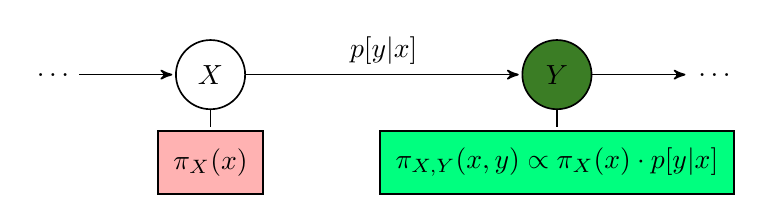
\begin{tikzpicture}[->,>=stealth',shorten >=1pt,auto,node distance=2.0cm,semithick]
                    
\node (X1) {$\ldots$}; 
\node[state](X2) [right of=X1] {$X$};
\node[state, fill=OliveGreen](X3) [right =3.5cm of X2] {$Y$};
\node (X4) [right of=X3] {$\ldots$};

\node[redbox][below=0.25cm of X2](P2){$\pi_{X}(x)$};               

\node[lgreenbox][below=0.25cm of X3](P3){$\pi_{X,Y}(x,y)\propto\pi_X(x)\cdot p[y|x]$};               
%
\path
	(X1) edge (X2)
	(X2) edge node[above]{$p[y|x]$}(X3)
	(X3) edge (X4);

\path
	(X2) edge[-] (P2)
	(X3) edge[-] (P3);



\end{tikzpicture}
\end{center}

\end{document}
